\documentclass[conference,letterpaper]{IEEEtran}

\usepackage[T1]{fontenc}
\usepackage{graphicx}
\usepackage{booktabs}
\usepackage{tabularx}
\usepackage{array}
\usepackage{xcolor}
\usepackage{amsmath}
\usepackage{cite}
\usepackage{url}
\usepackage{microtype}
\usepackage{listings}
% The default submission profile preserves metadata but emits neither bookmarks
% nor clickable annotations. Define \PaperReviewLinks before inputting this file
% only for an internal, link-enabled review copy.
\ifdefined\PaperReviewLinks
  \usepackage[hidelinks]{hyperref}
\else
  \usepackage[draft,bookmarks=false]{hyperref}
\fi
\usepackage{tikz}
\usetikzlibrary{arrows.meta,positioning,fit,calc,shapes.geometric,shapes.multipart,matrix,backgrounds}

% Centralized default conference profile. No venue-specific profile was supplied.
\newcommand{\paperTitle}{An AI-Based Platform for Content Summarization and Idea Generation using a Research Lab\textquoteright s Output}
\newcommand{\paperPdfTitle}{An AI-Based Platform for Content Summarization and Idea Generation using a Research Lab’s Output}
\newcommand{\paperAuthor}{Jarod Esareesingh}
\newcommand{\paperAffiliation}{Department of Computing \& Information Technology\\The University of the West Indies\\Trinidad and Tobago}
\newcommand{\paperEmail}{jarod.esareesingh@my.uwi.edu}
\newcommand{\paperSubject}{Design and controlled offline evaluation of a source-traceable research-intelligence and idea-generation platform}
\newcommand{\paperKeywords}{research intelligence, content summarization, idea generation, retrieval-augmented generation, reproducibility}

% The installed IEEE/Tectonic path does not expose a safe tagged-PDF alt-text
% primitive. Keeping descriptions beside figures makes the source auditable and
% ready for a venue toolchain that supports tagged PDF output.
\newcommand{\FigureDescription}[1]{}

% Generated by paper/scripts/generate_paper_assets.py; do not edit.
\newcommand{\PaperAiLabelBoundary}{AI-reviewed silver labels; no human inter-rater reliability or label-noise interval}
\newcommand{\PaperAiReviewedCount}{21}
\newcommand{\PaperCatalogCount}{134}
\newcommand{\PaperCorpusAbsenceCount}{1}
\newcommand{\PaperCorpusSnapshot}{corpus-04a010207327069a}
\newcommand{\PaperCpuModel}{AMD Ryzen 7 5800X 8-Core Processor}
\newcommand{\PaperDenseDimension}{384}
\newcommand{\PaperDenseModel}{sentence-transformers/all-MiniLM-L6-v2}
\newcommand{\PaperDenseModelDisplay}{\nolinkurl{sentence-transformers/all-MiniLM-L6-v2}}
\newcommand{\PaperDenseMrr}{0.939}
\newcommand{\PaperDenseMrrCi}{[0.842, 1.000]}
\newcommand{\PaperDenseNdcgTen}{0.939}
\newcommand{\PaperDenseNdcgTenCi}{[0.870, 0.994]}
\newcommand{\PaperDenseRecallTen}{0.989}
\newcommand{\PaperDenseRecallTenCi}{[0.968, 1.000]}
\newcommand{\PaperDenseRecallThree}{0.916}
\newcommand{\PaperDenseRecallThreeCi}{[0.821, 1.000]}
\newcommand{\PaperDenseRevision}{826711e54e001c83835913827a843d8dd0a1def9}
\newcommand{\PaperDenseRevisionDisplay}{\nolinkurl{826711e54e001c83835913827a843d8dd0a1def9}}
\newcommand{\PaperEligibleChunkCount}{719}
\newcommand{\PaperEligiblePaperCount}{96}
\newcommand{\PaperExternalDocumentCount}{3}
\newcommand{\PaperExternalTopOneCount}{3}
\newcommand{\PaperExtractionSignalCount}{1}
\newcommand{\PaperHashingDimension}{256}
\newcommand{\PaperHashingMrr}{0.588}
\newcommand{\PaperHashingMrrCi}{[0.412, 0.763]}
\newcommand{\PaperHashingNdcgTen}{0.582}
\newcommand{\PaperHashingNdcgTenCi}{[0.411, 0.745]}
\newcommand{\PaperHashingRecallTen}{0.704}
\newcommand{\PaperHashingRecallTenCi}{[0.509, 0.886]}
\newcommand{\PaperHashingRecallThree}{0.654}
\newcommand{\PaperHashingRecallThreeCi}{[0.443, 0.851]}
\newcommand{\PaperHeuristicHybridMrr}{0.813}
\newcommand{\PaperHeuristicHybridMrrCi}{[0.650, 0.947]}
\newcommand{\PaperHeuristicHybridNdcgTen}{0.829}
\newcommand{\PaperHeuristicHybridNdcgTenCi}{[0.691, 0.939]}
\newcommand{\PaperHeuristicHybridRecallTen}{0.917}
\newcommand{\PaperHeuristicHybridRecallTenCi}{[0.794, 1.000]}
\newcommand{\PaperHeuristicHybridRecallThree}{0.795}
\newcommand{\PaperHeuristicHybridRecallThreeCi}{[0.611, 0.947]}
\newcommand{\PaperHeuristicTermCount}{6}
\newcommand{\PaperIntentMismatchCount}{2}
\newcommand{\PaperKeywordMrr}{0.947}
\newcommand{\PaperKeywordMrrCi}{[0.868, 1.000]}
\newcommand{\PaperKeywordNdcgTen}{0.958}
\newcommand{\PaperKeywordNdcgTenCi}{[0.900, 0.998]}
\newcommand{\PaperKeywordRecallTen}{1.000}
\newcommand{\PaperKeywordRecallTenCi}{[1.000, 1.000]}
\newcommand{\PaperKeywordRecallThree}{0.939}
\newcommand{\PaperKeywordRecallThreeCi}{[0.866, 1.000]}
\newcommand{\PaperLogicalCpuCount}{16}
\newcommand{\PaperMemoryGiB}{3.8}
\newcommand{\PaperMismatchCount}{2}
\newcommand{\PaperNeedsReprocessCount}{27}
\newcommand{\PaperNoHeuristicsMrr}{0.947}
\newcommand{\PaperNoHeuristicsNdcgTen}{0.952}
\newcommand{\PaperNoHeuristicsRecallTen}{1.000}
\newcommand{\PaperNoTextCount}{36}
\newcommand{\PaperNoTopicMrr}{0.886}
\newcommand{\PaperNoTopicNdcgTen}{0.902}
\newcommand{\PaperNoTopicRecallTen}{0.978}
\newcommand{\PaperPdfCount}{98}
\newcommand{\PaperPerformanceAvailable}{1}
\newcommand{\PaperPerformanceFailedSamples}{0}
\newcommand{\PaperPerformanceProfile}{full}
\newcommand{\PaperPerformanceProvenance}{61378b9aa78a}
\newcommand{\PaperPerformanceRepetitions}{3}
\newcommand{\PaperPerformanceSourceCommit}{5ccf22ec39cb}
\newcommand{\PaperPerformanceStageCount}{17}
\newcommand{\PaperPossibleAuthorPairCount}{13}
\newcommand{\PaperQaAbstentionAccuracy}{0.920}
\newcommand{\PaperQaAbstentionAccuracyCi}{[0.840, 0.980]}
\newcommand{\PaperQaAnswerCoverage}{0.136}
\newcommand{\PaperQaAnswerCoverageCi}{[0.067, 0.211]}
\newcommand{\PaperQaAnswerModel}{sentence-overlap-v1}
\newcommand{\PaperQaAnswerPointCount}{81}
\newcommand{\PaperQaAnswerProvider}{offline\_extractive}
\newcommand{\PaperQaCaseCount}{50}
\newcommand{\PaperQaCitationAttachedCount}{400}
\newcommand{\PaperQaCitationCompleteness}{1.000}
\newcommand{\PaperQaCitationCompletenessCi}{[1.000, 1.000]}
\newcommand{\PaperQaCitationCorrectness}{0.625}
\newcommand{\PaperQaCitationCorrectnessCi}{[0.564, 0.691]}
\newcommand{\PaperQaClaimCount}{400}
\newcommand{\PaperQaCorrectCitationLinkCount}{250}
\newcommand{\PaperQaCoveredAnswerPointCount}{11}
\newcommand{\PaperQaIncorrectCitationLinkCount}{8}
\newcommand{\PaperQaMissingAnswerPointCount}{33}
\newcommand{\PaperQaPartialAnswerPointCount}{37}
\newcommand{\PaperQaPartialCitationLinkCount}{142}
\newcommand{\PaperQaPartialClaimCount}{2}
\newcommand{\PaperQaRetrievalMode}{hybrid\_current\_untuned\_heuristic}
\newcommand{\PaperQaReturnedCitationCount}{250}
\newcommand{\PaperQaSupport}{0.995}
\newcommand{\PaperQaSupportCi}{[0.987, 1.000]}
\newcommand{\PaperQaSupportedClaimCount}{398}
\newcommand{\PaperQaUnanswerableAbstention}{0.000}
\newcommand{\PaperQaUnanswerableAbstentionCi}{[0.000, 0.000]}
\newcommand{\PaperQaUnanswerableCount}{4}
\newcommand{\PaperQaUnsupported}{0.000}
\newcommand{\PaperQaUnsupportedCi}{[0.000, 0.000]}
\newcommand{\PaperQaUnsupportedClaimCount}{0}
\newcommand{\PaperQaUsedReturnedCitationCount}{148}
\newcommand{\PaperRawChunkCount}{735}
\newcommand{\PaperRecBaseline}{0.631}
\newcommand{\PaperRecDelta}{0.024}
\newcommand{\PaperRecDeltaCi}{[-0.024, 0.071]}
\newcommand{\PaperRecFull}{0.655}
\newcommand{\PaperRecommendationConfigurationCount}{22}
\newcommand{\PaperRecommendationFeasibilityPartialCount}{84}
\newcommand{\PaperRecommendationItemsPerArm}{84}
\newcommand{\PaperRecommendationPerturbationCount}{21}
\newcommand{\PaperRecommendationPlanPartialCount}{12}
\newcommand{\PaperRecommendationProfileCount}{28}
\newcommand{\PaperRetrievalAnswerableTestCount}{19}
\newcommand{\PaperRetrievalBootstrapRepetitions}{10000}
\newcommand{\PaperRetrievalCaseCount}{50}
\newcommand{\PaperRetrievalDevCount}{30}
\newcommand{\PaperRetrievalTestCount}{20}
\newcommand{\PaperRetrievalUnanswerableFalsePositive}{1.000}
\newcommand{\PaperRetrievalUnanswerableTestCount}{1}
\newcommand{\PaperReviewAnswerCount}{27}
\newcommand{\PaperReviewArtifactCount}{14}
\newcommand{\PaperReviewEventCount}{48}
\newcommand{\PaperReviewRecommendationCount}{7}
\newcommand{\PaperSectionAccuracy}{0.900}
\newcommand{\PaperSectionCaseCount}{40}
\newcommand{\PaperSourceCommit}{72ae7e5e0c7a}
\newcommand{\PaperSourceTree}{2fbadee3b66e}
\newcommand{\PaperTopicCaseCount}{60}
\newcommand{\PaperTopicControlledLabelCount}{39}
\newcommand{\PaperTopicDenseCoverage}{0.958}
\newcommand{\PaperTopicDenseFone}{0.521}
\newcommand{\PaperTopicDensePrecision}{0.417}
\newcommand{\PaperTopicDenseRecall}{0.694}
\newcommand{\PaperTopicDevCount}{36}
\newcommand{\PaperTopicLexicalCoverage}{0.875}
\newcommand{\PaperTopicLexicalFone}{0.556}
\newcommand{\PaperTopicLexicalPrecision}{0.652}
\newcommand{\PaperTopicLexicalRecall}{0.484}
\newcommand{\PaperTopicSupportedTestLabelCount}{26}
\newcommand{\PaperTopicTestCount}{24}
\newcommand{\PaperTopicVocabularyCount}{40}
\newcommand{\PaperTopicZeroGoldTestLabelCount}{14}
\newcommand{\PaperTunedDenseWeight}{0.80}
\newcommand{\PaperTunedHybridMrr}{0.860}
\newcommand{\PaperTunedHybridMrrCi}{[0.719, 0.974]}
\newcommand{\PaperTunedHybridNdcgTen}{0.871}
\newcommand{\PaperTunedHybridNdcgTenCi}{[0.744, 0.967]}
\newcommand{\PaperTunedHybridRecallTen}{0.925}
\newcommand{\PaperTunedHybridRecallTenCi}{[0.807, 1.000]}
\newcommand{\PaperTunedHybridRecallThree}{0.856}
\newcommand{\PaperTunedHybridRecallThreeCi}{[0.707, 0.974]}
\newcommand{\PaperTunedKeywordWeight}{0.10}
\newcommand{\PaperUnknownChunkCount}{199}
\newcommand{\PaperWorkingTreeDirty}{true}
% Explicit layout-only fallback; remediation-v2 has not produced a validated package.
% These values are placeholders, not experimental evidence and not submission-ready.
\newcommand{\VTwoEvidenceTier}{not available (v2 not run)}
\newcommand{\VTwoRunStatus}{not\_run}
\newcommand{\VTwoEvaluationId}{peer-review-remediation-v2}
\newcommand{\VTwoEvaluationSourceCommitPrefix}{not run}
\newcommand{\VTwoProtocolShaPrefix}{not run}
\newcommand{\VTwoFrozenDatasetShaPrefix}{not run}
\newcommand{\VTwoLockedEnvironmentShaPrefix}{not run}
\newcommand{\VTwoCorpusSnapshotId}{not run}
\newcommand{\VTwoCorpusSnapshotShaPrefix}{not run}
\newcommand{\VTwoTechnicalEligiblePapers}{not run}
\newcommand{\VTwoTechnicalEligibleChunks}{not run}
\newcommand{\VTwoKeywordIndexCompleteness}{not run}
\newcommand{\VTwoKeywordConfigurationShaPrefix}{not run}
\newcommand{\VTwoEvaluationScope}{not evaluated}
\newcommand{\VTwoPublicProjectionExercised}{no}
\newcommand{\VTwoExternalProviderInvoked}{no}
\newcommand{\VTwoQAProvider}{not run}
\newcommand{\VTwoQAModel}{not run}
\newcommand{\VTwoFinderProvider}{not run}
\newcommand{\VTwoFinderModel}{not run}
\newcommand{\VTwoTopicMethod}{not run}
\newcommand{\VTwoOCRProvider}{not run}
\newcommand{\VTwoOCRProviderVersion}{not run}
\newcommand{\VTwoQATestCases}{not run}
\newcommand{\VTwoQAAnswerabilityPrecision}{not run}
\newcommand{\VTwoQAAnswerabilityPrecisionCi}{not run}
\newcommand{\VTwoQAAnswerabilityRecall}{not run}
\newcommand{\VTwoQAAnswerabilityRecallCi}{not run}
\newcommand{\VTwoQAFalsePositiveRate}{not run}
\newcommand{\VTwoQAFalsePositiveRateCi}{not run}
\newcommand{\VTwoQAAbstentionRate}{not run}
\newcommand{\VTwoQAAbstentionRateCi}{not run}
\newcommand{\VTwoQACitationLocatorPrecision}{not run}
\newcommand{\VTwoQACitationLocatorPrecisionCi}{not run}
\newcommand{\VTwoQACitationCompleteness}{not run}
\newcommand{\VTwoQACitationCompletenessCi}{not run}
\newcommand{\VTwoQAAnswerPointCoverage}{not run}
\newcommand{\VTwoQAAnswerPointCoverageCi}{not run}
\newcommand{\VTwoFinderTestProfiles}{not run}
\newcommand{\VTwoFinderEvidenceHitAtThree}{not run}
\newcommand{\VTwoFinderEvidenceHitAtThreeCi}{not run}
\newcommand{\VTwoFinderFullHitAtThree}{not run}
\newcommand{\VTwoFinderFullHitAtThreeCi}{not run}
\newcommand{\VTwoFinderHitAtThreeDelta}{not run}
\newcommand{\VTwoFinderHitAtThreeDeltaCi}{not run}
\newcommand{\VTwoFinderEvidenceMRR}{not run}
\newcommand{\VTwoFinderEvidenceMRRCi}{not run}
\newcommand{\VTwoFinderFullMRR}{not run}
\newcommand{\VTwoFinderFullMRRCi}{not run}
\newcommand{\VTwoFinderMRRDelta}{not run}
\newcommand{\VTwoFinderMRRDeltaCi}{not run}
\newcommand{\VTwoFinderTemplateConformance}{not run}
\newcommand{\VTwoFinderFactSuggestionSeparation}{not run}
\newcommand{\VTwoFinderUnknownTimeRetention}{not run}
\newcommand{\VTwoFinderConstraintFidelity}{not run}
\newcommand{\VTwoTopicTestCases}{not run}
\newcommand{\VTwoTopicKnownPositiveRecall}{not run}
\newcommand{\VTwoTopicKnownPositiveRecallCi}{not run}
\newcommand{\VTwoTopicKnownPositiveCaseCoverage}{not run}
\newcommand{\VTwoTopicKnownPositiveCaseCoverageCi}{not run}
\newcommand{\VTwoTopicUnadjudicatedPredictionCount}{not run}
\newcommand{\VTwoTopicUnadjudicatedPredictionShare}{not run}
\newcommand{\VTwoOCRStatus}{not run}
\newcommand{\VTwoOCRCharacterErrorRate}{not run}
\newcommand{\VTwoOCRWordErrorRate}{not run}
\newcommand{\VTwoOCRExactMatch}{not run}
\newcommand{\VTwoOCRRepeatable}{not run}
\newcommand{\VTwoPackageStatus}{not completed or validated}
\newcommand{\VTwoManifestShaPrefix}{not available}
\newcommand{\VTwoValidationAttestationShaPrefix}{not available}

% Generated topic error rows; do not edit.
\newcommand{\PaperTopicErrorRows}{%
Agriculture & 2 & 1 & 0 & 0.667 & 1.000 \tabularnewline
Ai & 0 & 0 & 4 & 0.000 & 0.000 \tabularnewline
Clustering & 3 & 1 & 0 & 0.750 & 1.000 \tabularnewline
Energy & 1 & 0 & 2 & 1.000 & 0.333 \tabularnewline
Networks & 0 & 2 & 2 & 0.000 & 0.000 \tabularnewline
Rag & 2 & 0 & 0 & 1.000 & 1.000 \tabularnewline
}


\hypersetup{
  pdftitle={\paperPdfTitle},
  pdfauthor={\paperAuthor},
  pdfsubject={\paperSubject},
  pdfkeywords={\paperKeywords}
}
\AtBeginDocument{\special{pdf:docinfo <<
  /Title (\paperPdfTitle)
  /Author (\paperAuthor)
  /Subject (\paperSubject)
  /Keywords (\paperKeywords)
>>}}

\definecolor{Navy}{HTML}{16324F}
\definecolor{Blue}{HTML}{2266A5}
\definecolor{Teal}{HTML}{168C86}
\definecolor{Gold}{HTML}{C98B2E}
\definecolor{Slate}{HTML}{526273}
\definecolor{PaleBlue}{HTML}{EAF2F8}
\definecolor{PaleTeal}{HTML}{E7F5F2}
\definecolor{PaleGold}{HTML}{FBF3E3}
\newcolumntype{Y}{>{\raggedright\arraybackslash}X}
\setlength{\emergencystretch}{2em}
\setlength{\tabcolsep}{3.2pt}
\lstdefinestyle{evidencecode}{
  language=Python,
  basicstyle=\ttfamily\scriptsize,
  numbers=left,
  numberstyle=\tiny\color{Slate},
  stepnumber=1,
  numbersep=4pt,
  frame=single,
  rulecolor=\color{Slate!60},
  backgroundcolor=\color{PaleBlue!45},
  breaklines=true,
  showstringspaces=false,
  columns=fullflexible,
  keepspaces=true,
  xleftmargin=1.25em,
  framexleftmargin=0.9em,
  aboveskip=3pt,
  belowskip=3pt,
  captionpos=b
}

\title{\paperTitle}
\author{\IEEEauthorblockN{\paperAuthor}
\IEEEauthorblockA{\paperAffiliation\\\paperEmail}}

\begin{document}
\maketitle

\begin{abstract}
Publication lists expose outputs but do not answer full-text questions or help students formulate bounded, evidence-linked projects. We present an engineering case study of the TTLAB Research Intelligence Platform, combining content summarization, citation-bearing question answering, an evaluated structured Thesis Extension Finder, and a post-evaluation conversational Idea Generator. The latter validates model source aliases, distinguishes paper-informed ideas from general suggestions, and records local-model and retrieval provenance; it does not establish novelty or feasibility. Historical v1 evaluation found strong lexical retrieval but weak citation targeting, answer completeness, abstention, and recommendation-feasibility evidence. A prospectively frozen remediation-v2 package is \VTwoPackageStatus{} and binds code, a frozen technical corpus, configurations, raw outputs, and a deterministic validator. Its \VTwoEvidenceTier{} held-out results report answerability precision \VTwoQAAnswerabilityPrecision{} (CI \VTwoQAAnswerabilityPrecisionCi), exact-locator citation precision \VTwoQACitationLocatorPrecision{} (\VTwoQACitationLocatorPrecisionCi), and a Finder Hit@3 change of \VTwoFinderHitAtThreeDelta{} (\VTwoFinderHitAtThreeDeltaCi). Known-positive topic recall is \VTwoTopicKnownPositiveRecall{} (\VTwoTopicKnownPositiveRecallCi); OCR character error on a deterministic fixture is \VTwoOCRCharacterErrorRate{}. These metrics concern a \VTwoEvaluationScope{} corpus and do not evaluate the newer Idea Generator. Source traceability means inspectable locators and provenance, not entailment or factual correctness. No recruited participants or independent human validation establish advisory usefulness, novelty, feasibility, or supervisor fit.
\end{abstract}

\begin{IEEEkeywords}
research intelligence, content summarization, idea generation, retrieval-augmented generation, source traceability, reproducibility
\end{IEEEkeywords}

\section{Introduction}
Large scholarly indexes connect papers and people \cite{giles1998citeseer,tang2008arnetminer,priem2022openalex}, while recommender and expert-finding research supports content/profile matching \cite{beel2016researchpaper,balog2006formal}. A laboratory archive has a narrower but less forgiving problem: missing PDFs, uncertain identities, generated advice, and incomplete review must remain visible instead of being hidden behind a polished search box.

The TTLAB precursor collected and displayed publications, generated lay summaries and notifications, and supported manual podcast preparation; evaluated full-text RAG was future work \cite{narine2025automating}. We extend it with full-paper ingestion, content summarization, page-aware retrieval, citation-returning question answering, thesis-extension support, topic/author exploration, and correction records. The evaluated structured Finder ranks evidence-bearing papers before adding a labelled proposal. The current public Idea Generator instead supports bounded conversation and one to three schema-validated directions, but neither mode can establish novelty, data access, workload, or researcher availability.

Here \emph{source-traceable} means that an output retains paper, chunk, page/section, provider/model, time, warning, and review-state locators. Traceability is not entailment, completeness, factual correctness, feasibility, or endorsement. This distinction governs both the application and the claims below.

Three questions organize the study: \textbf{RQ1}, can a heterogeneous archive become an internally consistent corpus and how do retrieval modes compare; \textbf{RQ2}, how strong are evidence-linked answers, extension suggestions, topics, and author links under their stated constructs; and \textbf{RQ3}, how reproducible, reviewable, and responsibly bounded is the artefact? Contributions are a hash-bound corpus/index contract; a modular, evidence-first platform with typed idea-generation boundaries; a prospective source-derived protocol plus preserved negative historical evidence; and a sanitized reproduction boundary. No recruited participants were used, so usefulness and supervisor suitability remain untested.

\section{Related Work}
Scholarly discovery systems progressed from autonomous citation indexing to literature/author graphs and open entity catalogues \cite{giles1998citeseer,tang2008arnetminer,priem2022openalex}. Their scale is useful for discovery, but a small institutional system must also expose why a paper was included, which file supplied a passage, whether an identity is confirmed, and whether generated material has been reviewed. Research-paper recommendation surveys likewise show that methods, user models, and evaluation protocols vary widely \cite{beel2016researchpaper}; an evidence match is not the same as a feasible supervisory recommendation. Expert-finding models infer expertise from documents \cite{balog2006formal}, so our author links are deliberately phrased as publication-derived associations rather than availability or endorsement.

BM25-style lexical ranking remains a strong baseline \cite{robertson2009bm25}. Feature hashing is a memory-bounded sparse representation, not a learned semantic encoder \cite{weinberger2009featurehashing}. Sentence-BERT and DPR provide learned sentence/passage representations \cite{reimers2019sentencebert,karpukhin2020dpr}; BEIR cautions that rankings vary across tasks and domains \cite{thakur2021beir}. We therefore compare modes rather than presuming dense or hybrid superiority.

RAG conditions generation on retrieved evidence \cite{lewis2020rag}, and later work adds retrieval/self-critique controls \cite{asai2024selfrag}. Evaluation frameworks inspect context relevance and faithfulness \cite{es2024ragas,saadfalcon2024ares}; atomic decomposition exposes claim-level support \cite{min2023factscore}. Returned citations nevertheless can target the wrong passage, and high support can coexist with missing answer points. Topic interpretability likewise requires inspection rather than relying on aggregate coherence \cite{doogan2021topic}. Human-in-the-loop guidance motivates visible uncertainty and correctable outputs \cite{amershi2014power}.

\section{Methodology and System}
\subsection{Units, Corpus, and Evidence Boundary}
The study combines design-science-oriented artefact construction with controlled offline evaluation. Units are papers/chunks for corpus integrity; queries for retrieval; atomic claims, citation links, and expected answer points for QA; synthetic profiles and ranked paper sets for recommendation; papers/labels for topics; and executable stages for performance. TTLAB authorized the project and corpus use, but that is neither ethics-board approval nor blanket third-party redistribution permission.

Design decisions were mapped to observable failures. Deterministic import and hash-checked indexes address silent corpus drift; page locators and typed evidence address unverifiable generation; evidence-only Finder output addresses users who do not want generated advice; validated aliases and a general-suggestion state bound conversational ideas; append-only review events address untraceable correction; and explicit unavailable states address missing providers or PDFs. Each mechanism is evaluated at the narrowest valid unit instead of treating a passing user-interface test as retrieval evidence or a citation count as faithfulness.

The historical v1 snapshot starts with \PaperCatalogCount{} records and \PaperPdfCount{} available PDFs. A paper enters technical experiments only when metadata, a permitted PDF, extracted text, and title/content checks agree. Table~\ref{tab:corpus} shows that boundary: \PaperEligiblePaperCount{} papers and \PaperEligibleChunkCount{} of \PaperRawChunkCount{} chunks were eligible; \PaperNoTextCount{} records needed text/review, \PaperMismatchCount{} PDFs were mismatches, and \PaperUnknownChunkCount{} eligible chunks retained an Unknown section instead of a forced label. A \PaperSectionCaseCount{}-case AI-silver check measured \PaperSectionAccuracy{} section accuracy.

\begin{table}[t]
\caption{Historical v1 corpus and index boundary.}
\label{tab:corpus}
\centering
\scriptsize
\begin{tabular}{@{}lr@{\quad}lr@{}}
\toprule
Catalogue & \PaperCatalogCount & Local PDFs & \PaperPdfCount \\
Eligible papers & \PaperEligiblePaperCount & Needs text/review & \PaperNoTextCount \\
Raw chunks & \PaperRawChunkCount & Eligible chunks & \PaperEligibleChunkCount \\
PDF mismatches & \PaperMismatchCount & Unknown sections & \PaperUnknownChunkCount \\
\bottomrule
\end{tabular}
\end{table}

Keyword FTS, \PaperHashingDimension{}-dimensional signed feature hashing, and the pinned \PaperDenseDimension{}-dimensional \texttt{all-MiniLM-L6-v2} encoder share an ordered eligible-chunk boundary. Feature hashing is not labelled learned semantic retrieval. Manifests bind corpus/configuration hashes, model revision, dimensions, code, ordered source hashes, and completeness; startup and experiments reject stale or partial indexes. Historical artefacts retain their own execution identities instead of being relabelled as current.

Remediation-v2 is separately identity-bound to source commit \texttt{\VTwoEvaluationSourceCommitPrefix{}} and snapshot \texttt{\VTwoCorpusSnapshotId{}}. Its technical boundary contains \VTwoTechnicalEligiblePapers{} papers and \VTwoTechnicalEligibleChunks{} chunks. The package status is \VTwoPackageStatus{}. These generated values prevent a manuscript build from silently combining a new corpus with old results.

\subsection{Evaluation Protocol}
Historical v1 used \PaperRetrievalCaseCount{} source-derived retrieval cases, one AI process for source-linked labels, a later shuffled source-first reinspection without rankings, and a fixed \PaperRetrievalDevCount{}/\PaperRetrievalTestCount{} development/test split. On answerable queries, set recall is $|G_q\cap P_{q,k}|/|G_q|$; MRR and nDCG@10 complement it. Query-bootstrap intervals and Holm-corrected paired tests were reported, but correlated AI-label error was not modelled.

The prospective remediation protocol freezes its corpus, source-derived cases, locators, splits, configuration, environment lock, and output schema before execution. Cases were constructed from sources without consulting rankings; held-out outputs are immutable after the run. Ask uses fixed keyword retrieval, a deterministic extractive answerer, and a predeclared answerability rule over \VTwoQATestCases{} test cases. Claims are decomposed and scored for exact evidence locators, citation completeness, answer-point coverage, and abstention. Finder compares evidence-only ranking with full, separately labelled suggestions on the same retrieval response for \VTwoFinderTestProfiles{} held-out synthetic profiles. Profiles are proxies, not students.

Topics use \VTwoTopicTestCases{} source-derived, known-positive test cases. Because labels are not exhaustive, the protocol reports positive-label recall, coverage, and unadjudicated predictions---not precision, F1, or exact match. A deterministic raster fixture exercises the OCR path but is not a corpus OCR estimate. Cluster-level bootstrap intervals quantify sampling of cases, profiles, or papers only. A shuffled second AI pass records disagreements; repeated AI inspection is not independent human validation, inter-rater reliability, or entailment assessment.

\begin{figure*}[t]
\centering
\resizebox{0.96\textwidth}{!}{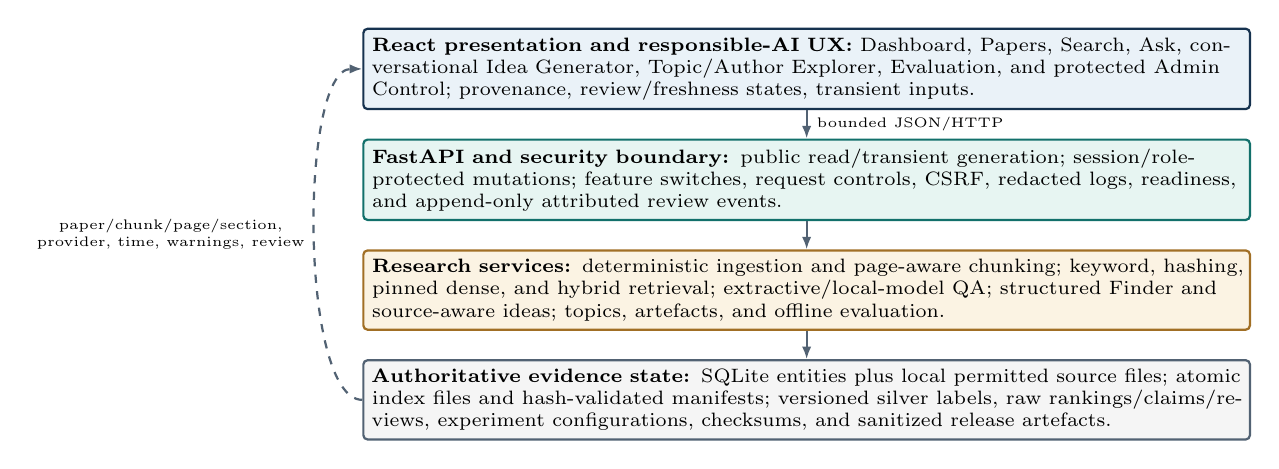
\begin{tikzpicture}[
  node distance=3.6mm,
  layer/.style={draw=Navy, rounded corners=1.5pt, thick, align=left, inner sep=3.2pt, text width=0.91\textwidth, font=\scriptsize},
  arr/.style={-{Latex[length=1.6mm]}, thick, draw=Slate}
]
  \node[layer, fill=PaleBlue] (ui) {\textbf{React presentation and responsible-AI UX:} Dashboard, Papers, Search, Ask, conversational Idea Generator, Topic/Author Explorer, Evaluation, and protected Admin Control; provenance, review/freshness states, transient inputs.};
  \node[layer, below=of ui, fill=PaleTeal, draw=Teal!80!black] (api) {\textbf{FastAPI and security boundary:} public read/transient generation; session/role-protected mutations; feature switches, request controls, CSRF, redacted logs, readiness, and append-only attributed review events.};
  \node[layer, below=of api, fill=PaleGold, draw=Gold!80!black] (logic) {\textbf{Research services:} deterministic ingestion and page-aware chunking; keyword, hashing, pinned dense, and hybrid retrieval; extractive/local-model QA; structured Finder and source-aware ideas; topics, artefacts, and offline evaluation.};
  \node[layer, below=of logic, fill=gray!8, draw=Slate] (data) {\textbf{Authoritative evidence state:} SQLite entities plus local permitted source files; atomic index files and hash-validated manifests; versioned silver labels, raw rankings/claims/reviews, experiment configurations, checksums, and sanitized release artefacts.};
  \draw[arr] (ui) -- node[right,font=\tiny]{bounded JSON/HTTP} (api);
  \draw[arr] (api) -- (logic);
  \draw[arr] (logic) -- (data);
  \draw[-{Latex[length=1.6mm]},thick,dashed,draw=Slate] (data.west) .. controls +(-8mm,0) and +(-8mm,0) .. node[left,font=\tiny,align=center]{paper/chunk/page/section,\\provider, time, warnings, review} (ui.west);
\end{tikzpicture}
}
\FigureDescription{Four layers connect the React interface, protected FastAPI boundary, research-intelligence services, and authoritative evidence state. A reverse arrow returns paper, chunk, page, provider, warning, and review metadata.}
\caption{Implemented architecture. Administrative mutations cross an authenticated boundary; evidence locators return through every layer.}
\label{fig:architecture}
\end{figure*}

\begin{figure*}[t]
\centering
\resizebox{0.96\textwidth}{!}{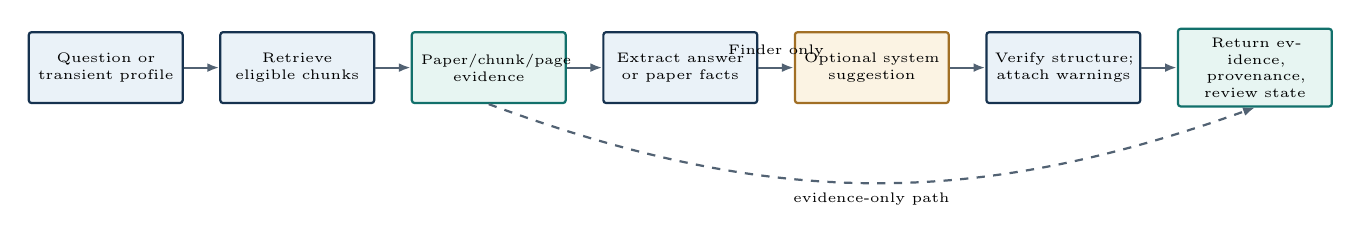
\begin{tikzpicture}[
  node distance=3.5mm and 4.5mm,
  box/.style={draw=Navy,rounded corners=1pt,thick,fill=PaleBlue,align=center,text width=17.2mm,minimum height=9mm,font=\tiny},
  rec/.style={box,fill=PaleGold,draw=Gold!80!black},
  store/.style={box,fill=PaleTeal,draw=Teal!80!black},
  arr/.style={-{Latex[length=1.5mm]},thick,draw=Slate}
]
  \node[box] (q) {Question or transient profile};
  \node[box, right=of q] (r) {Retrieve eligible chunks};
  \node[store, right=of r] (e) {Paper/chunk/page evidence};
  \node[box, right=of e] (a) {Extract answer or paper facts};
  \node[rec, right=of a] (s) {Optional system suggestion};
  \node[box, right=of s] (v) {Verify structure; attach warnings};
  \node[store, right=of v] (u) {Return evidence, provenance, review state};
  \draw[arr] (q) -- (r);
  \draw[arr] (r) -- (e);
  \draw[arr] (e) -- (a);
  \draw[arr] (a) -- node[above,font=\tiny]{Finder only} (s);
  \draw[arr] (s) -- (v);
  \draw[arr] (v) -- (u);
  \draw[-{Latex[length=1.5mm]},thick,dashed,draw=Slate] (e.south) to[bend right=20] node[below,font=\tiny]{evidence-only path} (u.south);
\end{tikzpicture}
}
\FigureDescription{A question, structured profile, or bounded idea conversation is retrieved against eligible chunks. Evidence feeds an answer, paper-fact record, or source-aware idea. The structured Finder retains an evidence-only path; the Idea Generator validates aliases and marks unmatched output as a general suggestion. Warnings and provenance return to the user.}
\caption{Ask, structured Finder, and conversational Idea Generator evidence flow.}
\label{fig:workflow}
\end{figure*}

Figures~\ref{fig:architecture} and \ref{fig:workflow} summarize the implementation. The React interface provides papers, search, Ask, Idea Generator, topic/author, evaluation, and protected Admin Control routes; the structured Finder remains an evaluated backend mode. It renders freshness, provider/model/time, warnings, review state, citations, and explicit empty, unavailable, and retry states. FastAPI separates public reads and transient generation from session/role-protected mutations; exact origins/hosts, bounded requests, safe file/URL handling, redacted logs, and append-only attributed review events are enforced. Public question, profile, and conversation inputs are non-persistent by default.

Page-aware extraction distinguishes blank, scanned, and mixed pages. Search returns mode, score components, pages, sections, freshness, and the active corpus identity. Runtime grounding checks locator presence and weak lexical overlap, not entailment. The answerer extracts bounded sentences. Finder first constructs source-backed baseline work, paper-stated future work, and an explicitly inferred gap; only then may it add a labelled suggestion. The Idea Generator retrieves at most six distinct paper sources, applies the fixed answerability gate, validates a one-to-three-idea JSON schema, and converts unrecognised aliases into an explicit unverified-source phrase. Ideas without a valid alias are marked \texttt{general\_suggestion}; cited papers are background, not novelty evidence.

Technical eligibility is not publication approval. Production public routes use a stricter projection requiring rights clearance, review, publication state, and an aligned public index generation. An explicit loopback-only demo may preview technically eligible records with visible insecure-demo and rights warnings; it does not change publication decisions. The remediation evaluation uses only the technical boundary and is not evidence of public behavior. Ollama did not contribute historical v1 or remediation-v2 results, so no response, quality, digest, or latency comparison was invented for those experiments; current runtime code performs pre/post digest checks and records incomplete response attestation.

\subsection{Evidence Contracts and Failure Semantics}
Derived state is generation-addressed. Extraction records bind exact PDF bytes; chunk records bind the extraction generation and exact UTF-8 text; each authoritative index manifest binds the ordered eligible source identities and active configuration. Reconciliation validates that chain before rebuilding. Index files are written as immutable generations, and the active pointer changes only after database status is committed. A bounded demo build cannot target the authoritative index. Startup and requests fail closed on a missing, partial, stale, or differently scoped manifest rather than silently falling back to another corpus.

Ask decomposes an answer into checkable claims, retains only citations used by those claims, and exposes an unsupported or abstained state when fixed answerability evidence is insufficient. A citation establishes a locator, not that the cited passage entails the prose. Finder ranks evidence-bearing papers before constructing suggestions; candidate facts are recomputed from the selected paper, while unresolved time, data, novelty, and feasibility remain unknown or assumptions. The public API omits technical hashes and local paths but retains safe paper/page/chunk navigation.

Review state is likewise typed. Corrections, review decisions, and the effective display projection remain separate; events are attributed and hash chained. An AI actor can record an AI-review outcome but cannot create a human approval. Provider-offline, stale-index, and empty-public-corpus states are first-class responses with retry or evidence-only paths. Table~\ref{tab:evidence-contracts} summarizes the permitted inference boundary.

\begin{table}[t]
\caption{Evidence contracts and prohibited inferences.}
\label{tab:evidence-contracts}
\centering
\scriptsize
\begin{tabularx}{\columnwidth}{@{}lYY@{}}
\toprule
Surface & Evidence retained & Does not establish \\
\midrule
Search & corpus, chunk, rank, mode & relevance truth \\
Ask & claim, locator, warning & entailment/correctness \\
Finder/ideas & fact, basis, suggestion & novelty/feasibility \\
Topics/authors & source links, review state & expertise/availability \\
Review & actor type, event chain & human approval by AI \\
\bottomrule
\end{tabularx}
\end{table}

The post-evaluation Idea Generator enforces the evidence boundary in \texttt{idea\_generator.py}. After aliases are checked against retrieved chunks, Listing~\ref{lst:idea-boundary} preserves only validated chunk identifiers and gives every other idea the \texttt{general\_suggestion} basis. This prevents an invented alias from becoming a displayed citation; it does not validate the idea itself.

\begin{lstlisting}[style=evidencecode,float=t,caption={Abridged Idea Generator evidence boundary.},label={lst:idea-boundary}]
if invalid_aliases:
    response_warnings.append(
        "Model source labels outside retrieved evidence were replaced."
    )
valid_aliases = list(dict.fromkeys(valid_aliases))
ideas.append({
    **draft_payload,
    "basis": ("paper_informed" if valid_aliases
              else "general_suggestion"),
    "source_chunk_ids": [
        str(alias_to_result[a].get("chunk_id") or "")
        for a in valid_aliases
    ],
})
\end{lstlisting}

\section{Results}
\subsection{RQ1: Historical v1 Corpus and Retrieval}
All three historical v1 indexes covered \PaperEligibleChunkCount{}/\PaperEligibleChunkCount{} eligible chunks; excluded/raw chunks could not enter that evaluation. Author cleanup removed navigation artefacts and repaired punctuation aliases, while \PaperPossibleAuthorPairCount{} possible same-person pairs remain unmerged pending external confirmation. Missing metadata stays empty.

\begin{table}[t]
\caption{Historical v1 held-out retrieval (\PaperRetrievalAnswerableTestCount{} answerable queries).}
\label{tab:retrieval}
\centering
\scriptsize
\begin{tabular}{@{}lrrrr@{}}
\toprule
Mode & R@3 & R@10 & MRR & nDCG@10 \\
\midrule
Keyword & \PaperKeywordRecallThree & \PaperKeywordRecallTen & \PaperKeywordMrr & \PaperKeywordNdcgTen \\
Feature hashing & \PaperHashingRecallThree & \PaperHashingRecallTen & \PaperHashingMrr & \PaperHashingNdcgTen \\
Learned dense & \PaperDenseRecallThree & \PaperDenseRecallTen & \PaperDenseMrr & \PaperDenseNdcgTen \\
Heuristic hybrid & \PaperHeuristicHybridRecallThree & \PaperHeuristicHybridRecallTen & \PaperHeuristicHybridMrr & \PaperHeuristicHybridNdcgTen \\
Dev-tuned hybrid & \PaperTunedHybridRecallThree & \PaperTunedHybridRecallTen & \PaperTunedHybridMrr & \PaperTunedHybridNdcgTen \\
\bottomrule
\end{tabular}
\end{table}

Table~\ref{tab:retrieval} shows that keyword had the highest historical point estimates: Recall@10 \PaperKeywordRecallTen{} (CI \PaperKeywordRecallTenCi) and MRR \PaperKeywordMrr{} (\PaperKeywordMrrCi). Dense MRR was \PaperDenseMrr{} (\PaperDenseMrrCi); tuned-hybrid MRR was \PaperTunedHybridMrr{} (\PaperTunedHybridMrrCi). No corrected comparison established hybrid superiority, and equivalence was not tested. Removing all \PaperHeuristicTermCount{} heuristics recovered Recall@10 \PaperNoHeuristicsRecallTen{} and MRR \PaperNoHeuristicsMrr{}. Every mode answered the single held-out unanswerable query, an unstable but adverse signal.

\subsection{RQ2: Historical Diagnosis and Prospective Evidence}
\begin{table}[t]
\caption{Historical v1 negative and null evidence.}
\label{tab:historical-diagnostics}
\centering
\scriptsize
\begin{tabularx}{\columnwidth}{@{}Yrr@{}}
\toprule
Outcome & Estimate/count & CI or denominator \\
\midrule
Citation correctness & \PaperQaCitationCorrectness & \PaperQaCitationCorrectnessCi \\
Strict answer-point coverage & \PaperQaAnswerCoverage & \PaperQaCoveredAnswerPointCount/\PaperQaAnswerPointCount; \PaperQaAnswerCoverageCi \\
Unanswerable abstention & \PaperQaUnanswerableAbstention & \PaperQaAbstentionCount/\PaperQaUnanswerableCount; \PaperQaUnanswerableAbstentionCi \\
Finder relevance change & \PaperRecDelta & \PaperRecDeltaCi \\
Finder full-mode return & \PaperRecommendationFullReturnedCount/\PaperRecommendationRequestedSlotCount & \PaperRecommendationFullReturnCoverage; \PaperRecommendationFullMissingCount{} missing \\
\bottomrule
\end{tabularx}
\end{table}

Table~\ref{tab:historical-diagnostics} summarizes the principal historical negatives. Historical v1 classified \PaperQaSupportedClaimCount{}/\PaperQaPartialClaimCount{}/\PaperQaUnsupportedClaimCount{} of \PaperQaClaimCount{} extractive claims as supported/partial/unsupported, yet strict answer-point coverage was only \PaperQaAnswerCoverage{} (\PaperQaCoveredAnswerPointCount/\PaperQaAnswerPointCount), and just \PaperQaAbstentionCount/\PaperQaUnanswerableCount{} unanswerable cases abstained (\PaperQaAnsweredCount/\PaperQaCaseCount{} cases answered overall). Its case-bootstrap intervals exclude AI-label uncertainty. Finder evidence-only mode returned \PaperRecommendationEvidenceReturnedCount/\PaperRecommendationRequestedSlotCount{} items, whereas full mode returned \PaperRecommendationFullReturnedCount/\PaperRecommendationRequestedSlotCount{}, leaving \PaperRecommendationFullMissingCount{} cutoff slots scored as zero; the relevance change was negative and its interval spanned zero. Conditional on the \PaperRecommendationFullReturnedCount{} returns, source fidelity passed \PaperRecommendationFullReturnedCount/\PaperRecommendationFullReturnedCount; pass/partial/fail counts were feasibility \PaperRecommendationFeasibilityPass/\PaperRecommendationFeasibilityPartial/\PaperRecommendationFeasibilityFail, MVP \PaperRecommendationMvpPass/\PaperRecommendationMvpPartial/\PaperRecommendationMvpFail, and evaluation plan \PaperRecommendationPlanPass/\PaperRecommendationPlanPartial/\PaperRecommendationPlanFail; separation passed/failed \PaperRecommendationSeparationPass/\PaperRecommendationSeparationFail, while usefulness failed \PaperRecommendationUsefulnessFail/\PaperRecommendationFullReturnedCount. Feasibility failure records unverified data, time, and skills, not known infeasibility. Topic silver evidence bound through \PaperTopicBindingExactCount{} exact chunk IDs and \PaperTopicBindingReboundCount{} deterministic same-paper locator rebound; \PaperTopicBindingDriftCount{} snapshot-drift binding preserved the persisted excerpt exactly. Binding integrity does not establish label correctness. These are AI-reviewed silver findings.

\begin{table}[t]
\caption{Prospective held-out technical outcomes (generated macros).}
\label{tab:prospective-results}
\centering
\scriptsize
\begin{tabularx}{\columnwidth}{@{}Yrr@{}}
\toprule
Outcome & Estimate & Cluster CI \\
\midrule
QA cases & \VTwoQATestCases & -- \\
Answerability precision & \VTwoQAAnswerabilityPrecision & \VTwoQAAnswerabilityPrecisionCi \\
Exact-locator citation precision & \VTwoQACitationLocatorPrecision & \VTwoQACitationLocatorPrecisionCi \\
Strict answer-point coverage & \VTwoQAAnswerPointCoverage & \VTwoQAAnswerPointCoverageCi \\
Finder profiles & \VTwoFinderTestProfiles & -- \\
Finder Hit@3 change & \VTwoFinderHitAtThreeDelta & \VTwoFinderHitAtThreeDeltaCi \\
Topic cases & \VTwoTopicTestCases & -- \\
Known-positive topic recall & \VTwoTopicKnownPositiveRecall & \VTwoTopicKnownPositiveRecallCi \\
OCR fixture character error & \VTwoOCRCharacterErrorRate & -- \\
\bottomrule
\end{tabularx}
\end{table}

Table~\ref{tab:prospective-results} is populated only from the validated package. Ask metrics test the fixed answerability gate and exact frozen locators; they do not establish factual correctness or entailment. Comparison of historical strict coverage \PaperQaAnswerCoverage{} (\PaperQaAnswerCoverageCi) with \VTwoQAAnswerPointCoverage{} (\VTwoQAAnswerPointCoverageCi) is descriptive and non-paired because the protocols use distinct frozen cases. The paired Finder delta is reported without a superiority claim, while template checks establish a data-contract property rather than project usefulness. Topic recall applies only to listed known positives; other predictions remain unadjudicated. OCR character error applies only to the deterministic fixture. All are \VTwoEvidenceTier{} technical-corpus judgments without human validation. Author links remain publication-derived associations, unresolved identities remain separate, and AI review events cannot confer human approval.

\subsection{RQ3: Reproduction and Operational Boundary}
The historical v1 local profile measured \PaperPerformanceStageCount{} process-cold/warm stages at concurrency one with \PaperPerformanceFailedSamples{} failures. Network discovery dominated variability and dense indexing dominated local compute/memory; OS caches were not flushed, so these medians are neither load nor capacity evidence. An external harness reacquired \PaperExternalDocumentCount{} pinned CC BY JATS/XML papers and obtained \PaperExternalTopOneCount{}/\PaperExternalDocumentCount{} fixed lexical top-one matches; that establishes format compatibility and trivial discrimination only, not cross-domain quality or PDF ingestion. The prospective package records source commit \texttt{\VTwoEvaluationSourceCommitPrefix{}}, corpus snapshot \texttt{\VTwoCorpusSnapshotId{}}, raw outputs, configuration, environment lock, and validation attestation. Exact full-corpus reruns still require lawful PDF and pinned-model access.

\section{Discussion, Threats, and Ethics}
The principal result is an evidence boundary, not a new ranking algorithm. Historical v1 showed that complete indexing and extractive support could coexist with weak citation choice, answer completeness, abstention, and Finder feasibility. The prospective measures narrow those constructs to a fixed answerability gate, exact source locators, paired recommendation ranks, known-positive topics, and a pipeline fixture. They do not erase the historical failures or convert contract conformance into benefit. Human studies must test usefulness, novelty, workload, and trust.

\subsection{Evidence-Driven Design Decisions}
The historical retrieval evidence makes keyword the defensible default for that snapshot: it had the strongest held-out point estimates and simple failure semantics. Dense search remains an explicit paraphrase-oriented alternative, not a claim of semantic quality. The tuned hybrid remains experimental because neither paired analysis nor ablations justified superiority. A future router must earn its complexity on a new locked test set.

QA therefore needs a multi-dimensional result state. A response can be source-derived but answer the wrong intent, cite an off-target passage, omit expected points, or answer when evidence is insufficient. The interface separates answerability, claim support, citation use, and completeness, and does not project aggregate scores onto a live answer. If the fixed gate fails, ranked evidence or an explicit unsupported state is safer than composed text.

Idea generation needs the analogous boundary. Ranking a paper can be justified by passages, interests, and stated constraints; proposing a thesis adds novelty, access, workload, skills, and evaluation assumptions the corpus cannot settle. The structured Finder distinguishes baseline work, paper-stated future work, inferred gap, and suggestion, while its evidence-only mode bypasses generation. The conversational Idea Generator instead reports a validated paper-informed/general basis and requires supervisor and literature review. Its four formative regression prompts and contract tests are not a quality or usefulness evaluation. No recommendation is supervisor-approved until an authorized human records that state.

Administrative review is an append-only evidence event rather than a silent overwrite. Local admin accounts use Argon2id, HttpOnly sessions, CSRF validation, expiry and lockout; service actors remain available for bounded automation. Bulk approval and publication require an actor-bound, ten-minute preview hash and reject changed state before appending review events. AI actors can mark AI-reviewed or needs-reprocess states but cannot impersonate human approval. These controls are local-application safeguards, not an institutional identity or production-operations claim.

The external smoke test and performance profile answer deployment questions only narrowly. The former shows that three licensed XML documents can enter the chunk contract and be separated by obvious lexical queries; it does not validate another discipline, language, or PDF path. The latter identifies expensive stages for a single local operator but offers no arrival-rate, tail-latency-under-load, or capacity evidence. Production planning must add representative traffic, concurrent users, failure injection, monitoring, and recovery tests without reusing these single-user medians as service-level objectives.

Construct validity is limited by AI-silver labels, source-derived positive-only topics, synthetic-profile proxies, and a fixture rather than corpus OCR. One AI procedure performs both shuffled passes, so correlated error remains and intervals exclude label uncertainty. Historical internal validity is limited by small test sets, one retrieval unanswerable, descriptive ablations, and a deterministic answerer; prospective cases remain small and source-derived. The post-evaluation Idea Generator has contract tests but no live-model quality, novelty, feasibility, or human-usefulness study. External validity is limited to one English-language laboratory snapshot and local hardware. Reproducibility remains bounded by lawful PDF/model access, network discovery, and OS caches.

TTLAB authorized project and corpus use. No participants were recruited and no ethics approval or exemption is claimed. Authorization does not transfer redistribution rights: PDFs, live database, derived text, secrets, model caches, and private prompts are excluded from the sanitized release. Public deployment additionally requires authenticated review, controlled origins, rate limits, monitoring, correction paths, backups, and accessibility validation. Datasheet, model-card, and risk-management practices inform disclosure \cite{gebru2021datasheets,mitchell2019modelcards,tabassi2023airmf}. OpenAI Codex supported repository inspection, test and silver-label preparation, targeted implementation, and focused editing; it was not a human assessor, and the author retained responsibility for design, interpretation, verification, and the manuscript. The current Tectonic PDF is intentionally not claimed as tagged PDF or PDF/UA; figure descriptions remain in source for a capable venue toolchain.

\section{Availability and Conclusion}
The sanitized bundle contains code, permitted metadata, sanitized experimental records, configurations, figure sources, manifests, hashes, and reproduction instructions. It excludes restricted content and is not the publisher package. Historical v1 negative and null findings remain alongside the \VTwoPackageStatus{} prospective evidence rather than being overwritten. The newer results apply to a \VTwoEvaluationScope{} corpus, with public projection exercised: \VTwoPublicProjectionExercised{}. The subsequently implemented Idea Generator demonstrates a traceable, failure-explicit software contract, not measured advisory improvement. The artefact is a source-traceable research-intelligence prototype, not a validated academic advisor: human utility, identity decisions, PDF rights, deployment controls, and venue compliance remain external validations.

\bibliographystyle{IEEEtran}
\IEEEtriggeratref{16}
\bibliography{../thesis/references}
\end{document}
